\documentclass[12pt]{elsarticle}
%\documentclass{amsart}
\usepackage{graphicx}
\usepackage{subfigure}
%\usepackage[nobysame]{amsrefs} % load package to handle bibliography
\usepackage{amssymb}


\makeatletter
\def\ps@pprintTitle{%
\let\@oddhead\@empty
\let\@evenhead\@empty
\def\@oddfoot{\reset@font\hfil\thepage\hfil}
\let\@evenfoot\@oddfoot
}
\makeatother

\title{3D CT Cone Beam Reconstruction Via Fan to Parallel Rebinning}
\author{Gregory Handy} 

\begin{document}
\maketitle

\section{Overview}


This semester (Fall 2012), I spent time reading and implementing the paper by Grass et al.\ titled ``3D cone-beam CT reconstruction for circular trajectories''. This paper presented a new reconstruction algorithm that modifies the well-known Feldkamp algorithm. Their new method can be broken into two major steps. The first step rebins the standard 3D cone beam geometry into a parallel-beam geometry along the source trajectory. It is possible to perform a filtered backprojection of the data at this step, and this method is known as P-FDK (parallel-FDK). Despite the algorithmic differences with FDK, this method does not differ in image quality/artifacts. The second step interpolates the projections onto a rectangular virtual detector plane and then proceeds with the filtered backprojection. This method is known as T-FDK (tent-FDK) and shows improved image quality.

In this paper I will provide a mathematical formalism of the algorithm, which is not found in the Grass et al.\ paper, along with directions on how to use the corresponding code. The formulas will be consistent with the variables used in the book chapters written by Fessler, and will reference sections out of these chapters, code found in the irt toolbox, as well as new code. The P-FDK and T-FDK methods have been completely implemented, but both should be tested on additional phantoms and real datasets. 


\section{P-FDK}
Assume that we are given cone-beam projection data $p^f(s,t,\beta)$, where
$f$ denotes the cone/fan-beam geometry, $s$ is the column position on the detector, $t$ is the row position on the detector, and $\beta$ is the angular position of the x-ray source. Rebinning to parallel fixes $t$, and rebins in the $s$ direction. For each fixed $t$, we are in the geometry presented in Section 3.9.

\subsection{Fan to Parallel Rebinning}

In Section 3.9.1, fan to parallel rebinning is defined assuming $r_{\mathrm{off}}=0$. We will also assume that we are using third-generation X-ray CT systems ($D_\mathrm{fs}=0$). This simplifies expression
(3.9.11) to
\begin{eqnarray*}
p^p(r,\phi) = p^f(D_{sd}\arcsin(r/D_{s0}),\phi-\arcsin(r/D_{s0})),
\end{eqnarray*}
where $\phi$ denotes the angle between the ray and the y-axis, $r$ is the distance from the center of rotation to the ray, $D_{s0}$ is the distance from the source to the center of rotation, and $D_{sd}$ is 
the distance from the source to the detector. This geometry can be seen in Figure \ref{fig:above}. Extending this to our 3D case yields, 
\begin{eqnarray*}
p^p(r,t,\phi) = p^f(D_{sd}\arcsin(r/D_{s0}),t,\phi-\arcsin(r/D_{s0})).
\end{eqnarray*}
The code implementing this step simply loops over the $t$-coordinate and makes repeated calls to the function rebin\_fan2par. It should be noted that this function requires a 2D projection matrix and a 2D CT geometry. Both of these can be created using the 3D CT geometry and 3D projection matrix provided. The user has control over the resulting parallel beam geometry (can change orbit, ds, etc.). These changes may offer a slight improvement in image quality. When decreasing ds to make a finer grid, the only requirement is that ds$\cdot$ns remains constant. 

After rebinning, one must define a new 3D CT geometry, and make any necessary changes (new ds, etc.). When doing so, the user should use the function ct\_geom\_par. This is essentially the same as ct\_geom, but allows for one additional variable, called `rebinned', which should now be set to 1. In the future, the ct\_geom code should be rewritten to allow for a new type, called par\_rebinned, but for now, the modified code checks if cg.rebinned == 1. This small change allows for our 3D CT geometry to use variables such as D$_\mathrm{sd}$, which can only be set to `inf' for the parallel type currently.


\subsection{New Geometry}
In order to complete the reconstruction algorithm, the new geometry must be understood. Figure \ref{fig:above} offers an above view of the rebinnned projection data while Figure \ref{fig:side}
offers a side view. The distances in these figures will be referenced in the following sections.

It is important to note that the total distance from the source to the detector (D$_\mathrm{sd}$) is kept 
constant. As a result, the `new' detector has an inverted


\begin{figure}[tbh]
\centering
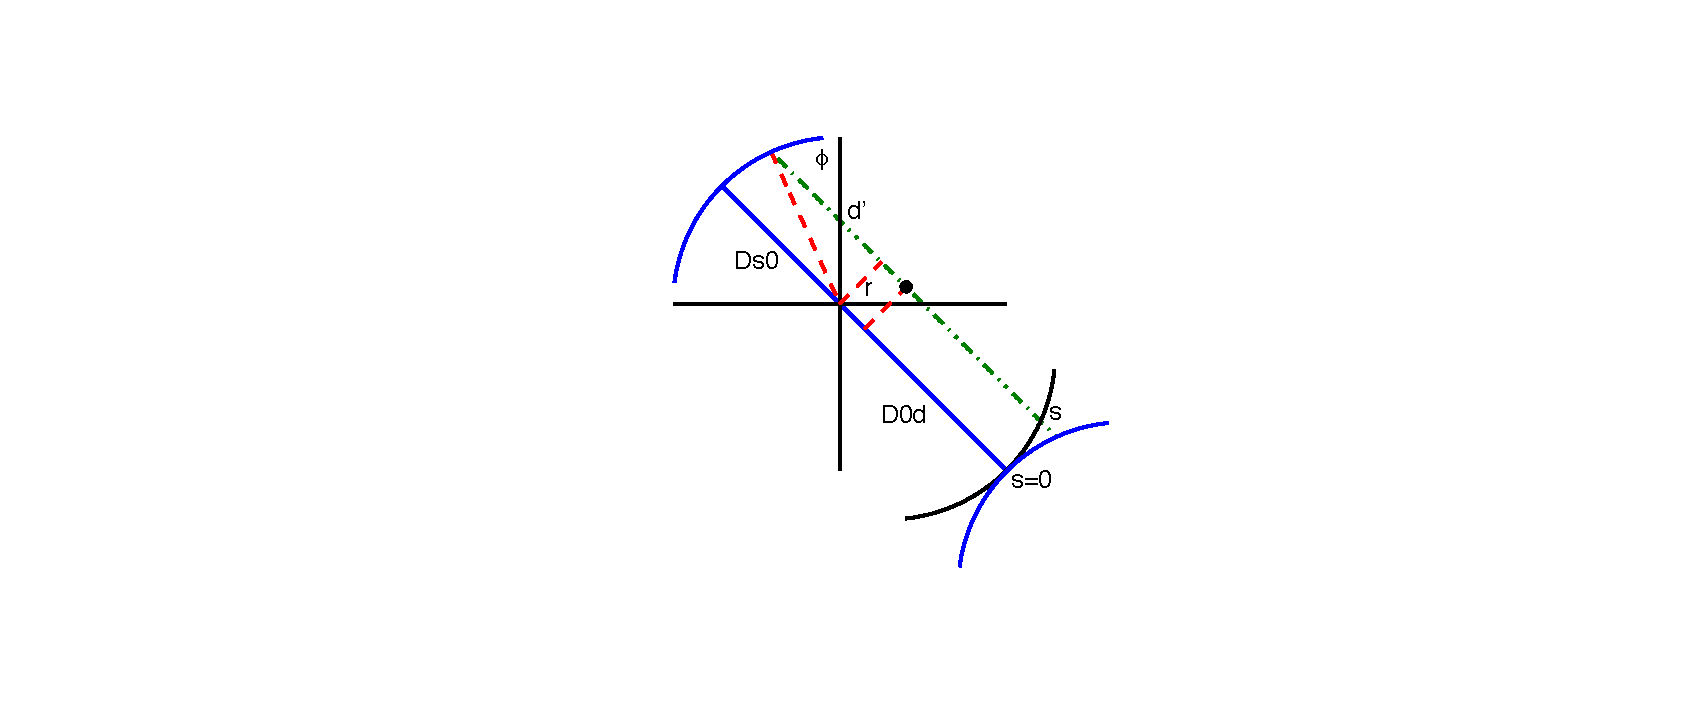
\includegraphics[scale=0.8]{Figures/officialAbove.pdf}
\caption{New geometry after rebinning. View is from above, and the x-y axis is provided. Note that the 
total distance D$_\mathrm{sd}$ is preserved for the rebinned data, which causes the new detector 
to curve outwards. Point of interest is the black dot.}
\label{fig:above}
\end{figure}

\begin{figure}[tbh]
\centering
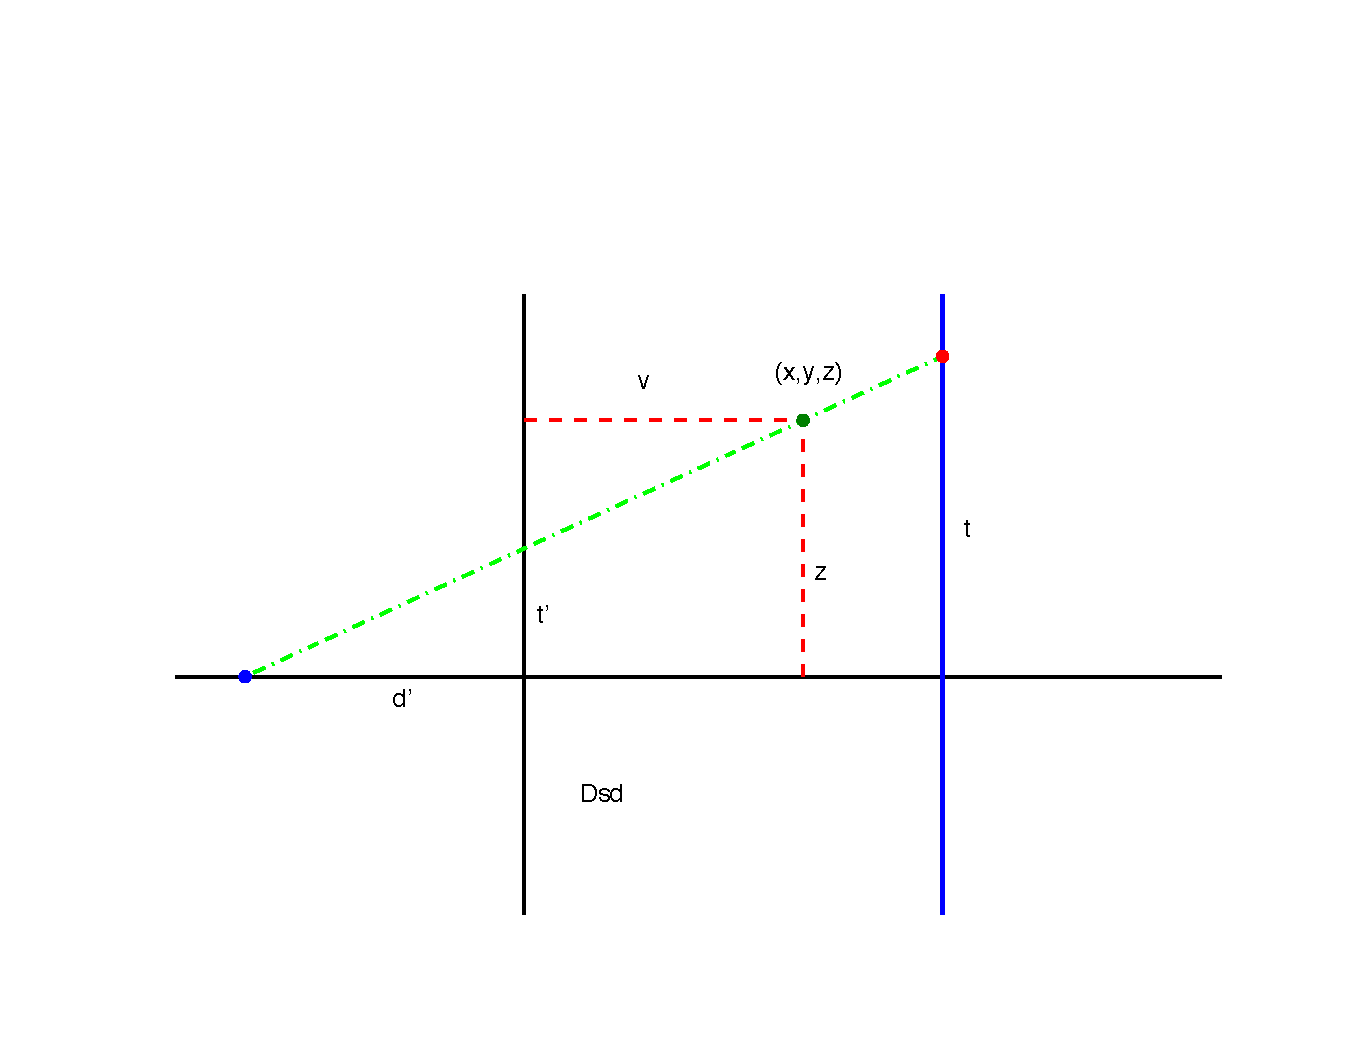
\includegraphics[scale=0.6]{Figures/officialSide.pdf}
\caption{The side view of the projection ray through the point of interest for the new geometry. The v-z axis is provided. The
total horizontal distance from the source to the detector is D$_\mathrm{sd}$.}
\label{fig:side}
\end{figure}
\clearpage 
\noindent arc. Figure \ref{fig:side} is given relative to the v-z
axis, where $v(x,y,\phi) = y_\phi$, which can be found in Equation (3.9.16), and is reproduced below:
\begin{eqnarray*}
v(x,y,\phi) = (-x \sin(\phi) + y \cos(\phi)).
\end{eqnarray*} 

\subsection{Filtered Backprojection}
The pre-weighting and filtering step proceed as normal with
\begin{eqnarray*}
w^p(t) &=& \frac{D_\mathrm{sd}}{\sqrt{D_\mathrm{sd}^2 + t^2}} \\
\hat{p}^p(r,t,\phi) &=& \Big(w^p(t) p^p(r,t,\phi)\Big) * g^p(r).
\end{eqnarray*}
The cosine weighting function can be derived from Figure \ref{fig:side}, and $g^p(r)$ is the usual
ramp filter used in the parallel-beam case (Equation (3.4.14)).

The backprojection now follows with
\begin{eqnarray*}
f_p(x,y,z) = \int_0^{2\pi} \hat{p}^p(r(x,y,\phi),t(x,y,z),\phi) d\phi,
\end{eqnarray*}
where
\begin{eqnarray*}
r(x,y,\phi) &=& x \cos(\phi) + y \sin(\phi) \\
t(x,y,z,\phi) &=& \frac{D_\mathrm{sd}z}{\sqrt{D_\mathrm{s0}^2-r(x,y,\phi)^2}+v(x,y,\phi)}. \
\end{eqnarray*}
The formula for $r(x,y,\phi)$ follows directly from the parallel beam geometry. In order to derive 
$t(x,y,z,\phi)$, note that by the similar triangles seen in Figure \ref{fig:side}, we have 
\begin{eqnarray*}
\frac{t}{D_\mathrm{sd}} &=& \frac{z}{d'+v}, \
\end{eqnarray*}
where
\begin{eqnarray*}
d'&=& \sqrt{D_\mathrm{s0}^2-r^2}, \
\end{eqnarray*}
can be derived from Figure \ref{fig:above}. It is interesting to note that additional weighting is not
required during the backprojection step. Figure \ref{fig:comp} shows the reconstruction results using
the P-FDK and FDK algorithms. 

\begin{figure}[tbh]
\centering
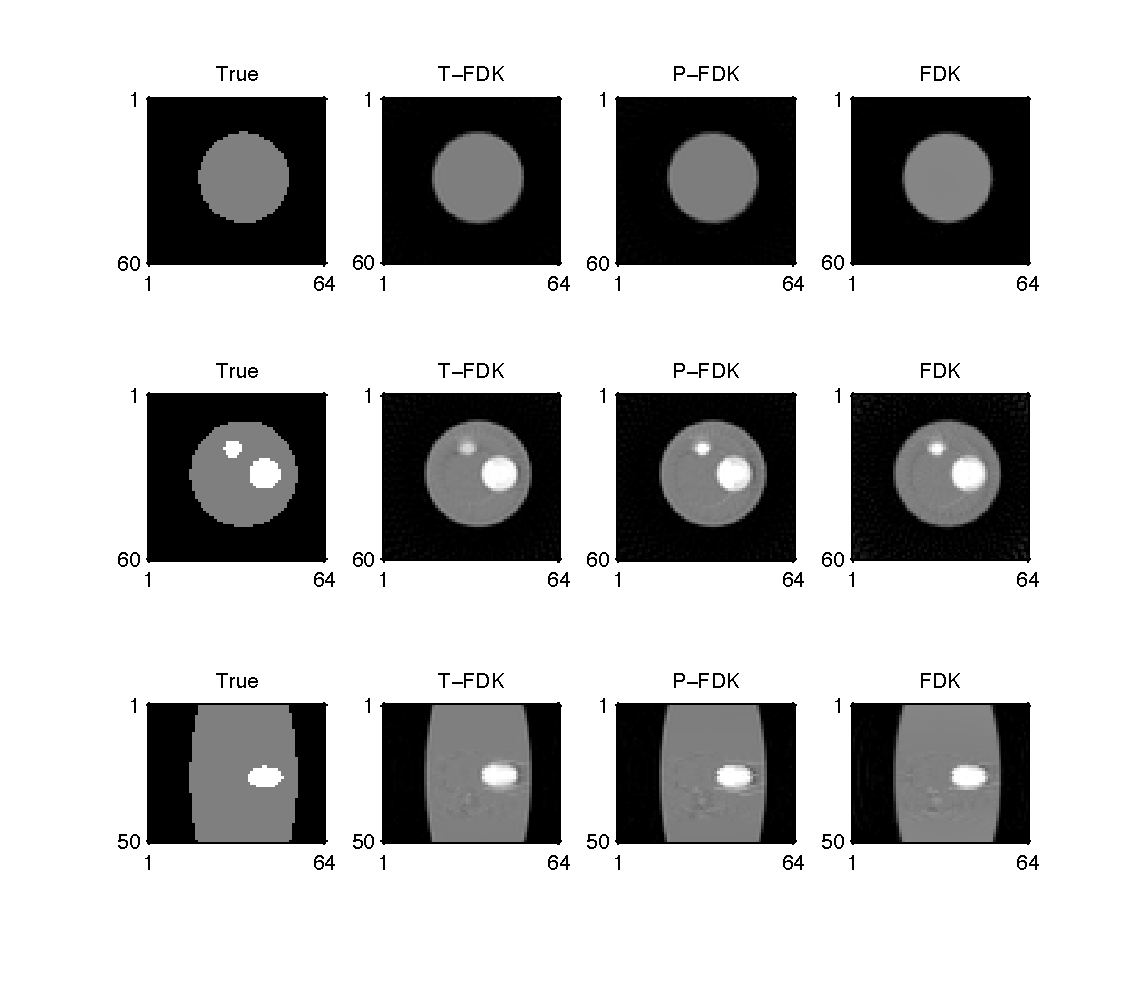
\includegraphics[scale=0.6]{Figures/comparison.pdf}
\caption{True and reconstruct images of a phantom for the first and middle slices, along with a side
view of the phantom.}
\label{fig:comp}
\end{figure}

\section{T-FDK}
Instead of filtering and backprojecting after rebinning to the parallel geometry, the T-FDK method interpolates the projection data to form a Cartesian grid for the projection data on a virtual detector found at the axis of rotation. Before interpolation, the grid at this virtual detector can be seen in Figure \ref{grid}. Instead of simply interpolating (in the vertical direction) a rectangle that is contained within this curved grid, we are interested in extrapolating in order to create a rectangle that contains the curved grid.

\begin{figure}[tbh]
\centering
\mbox{\subfigure{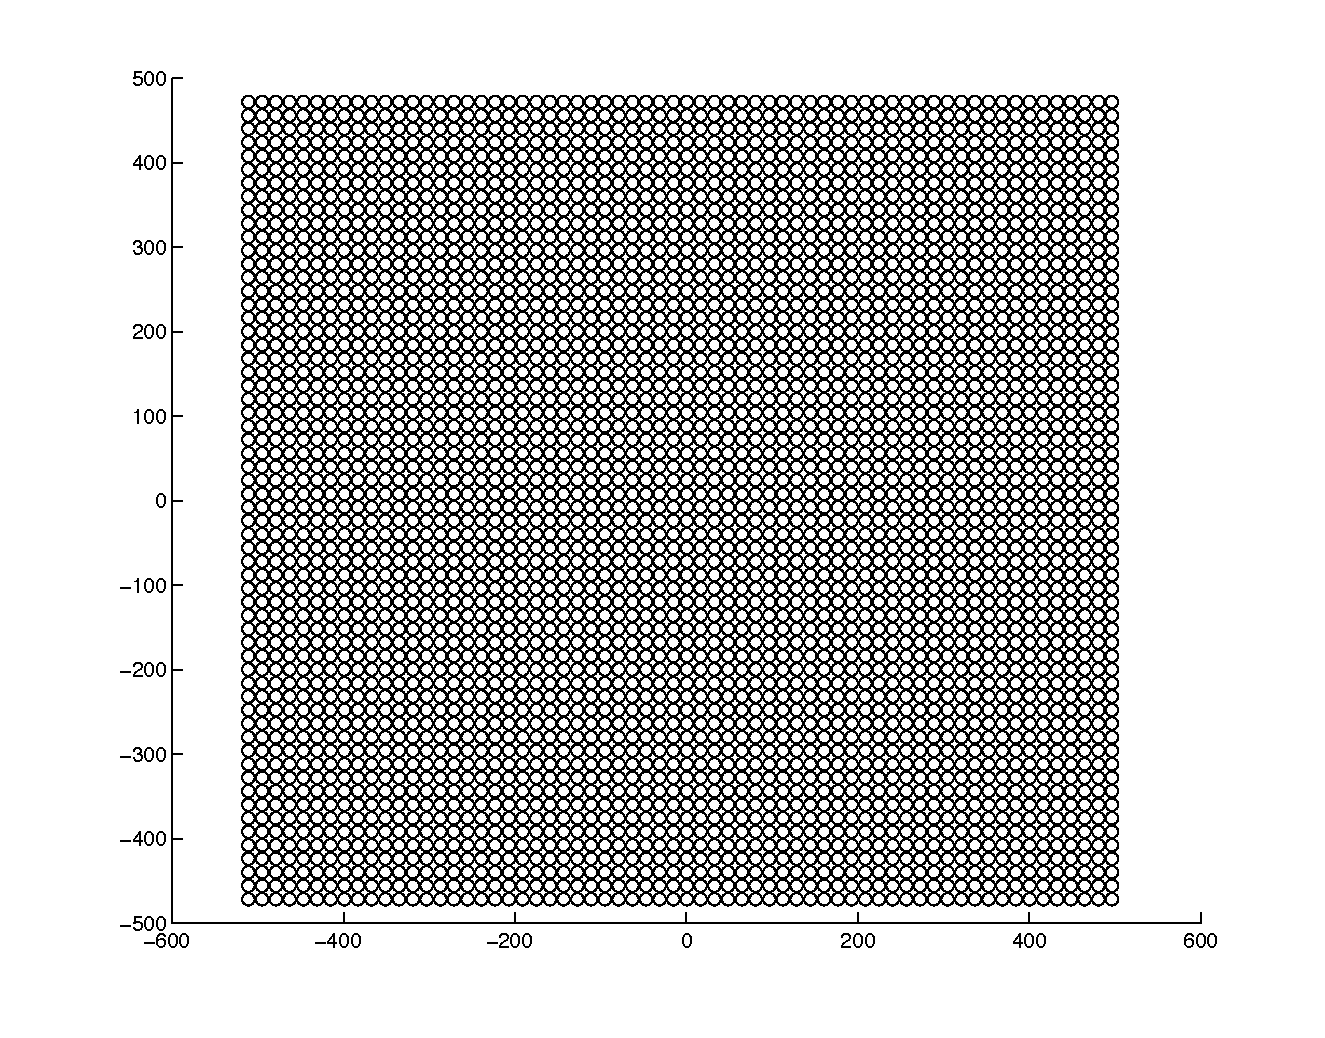
\includegraphics[width=2in]{Figures/rectGrid.pdf}
\quad
\subfigure{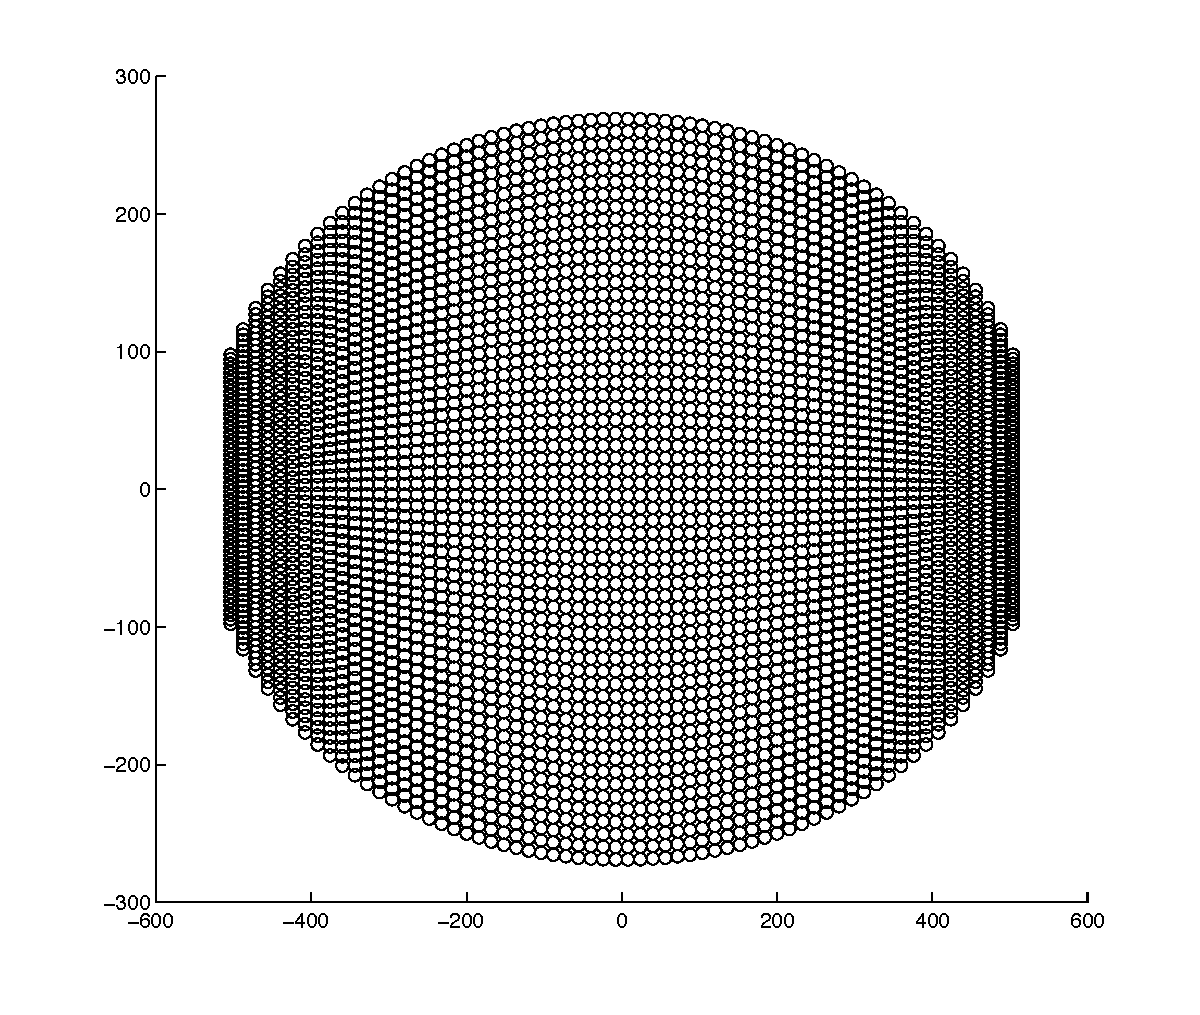
\includegraphics[width=2in]{Figures/curved.pdf} }}}
\caption{The left figure represents the projection grid on the detector, while the right figure represents the
same grid on the virtual detector located at the center of rotation.}
\label{grid}
\end{figure}

The function gridding.m performs this interpolation/extrapolation. It takes in the CT geometry and the
projection matrix, and returns the new projection matrix, along with coordinates for the new grid. This
function uses interp1 and currently performs linear interpolation, but this method can be changed.
We will refer to the new projection after interpolation/extrapolation in the $t$-direction as $p^{pr}(r,t',\phi)$.

After performing the interpolation/extrapolation, the algorithm continues with pre-weighting
and filtering, according to the equations
\begin{eqnarray*}
w^{pr}(r,t') &=& \frac{\sqrt{D_\mathrm{s0}^2-r^2}}{\sqrt{D_\mathrm{s0}^2 -r^2+ t'^2}} \\
\hat{p}^{pr}(r,t',\phi) &=& \Big(w^{pr}(r,t') p^{pr}(r,t',\phi)\Big) * g^p(r).
\end{eqnarray*}
The new cosine weighting function, $w^{pr}(r,t')$, can be derived directly from Figure \ref{fig:side}. 
Finally, the backprojection occurs with
\begin{eqnarray*}
f_{pr}(x,y,z) = \int_0^{2\pi} \hat{p}^{pr}(r(x,y,\phi),t'(x,y,z),\phi) d\phi,
\end{eqnarray*}
where $r(x,y,\phi)$ is the same as before, and
\begin{eqnarray*}
t'(x,y,z,\phi) &=& \frac{z\sqrt{D_\mathrm{s0}^2-r(x,y,\phi)^2}}{\sqrt{D_\mathrm{s0}^2-r(x,y,\phi)^2}+v(x,y,\phi)}. \
\end{eqnarray*}
Again, this follows from the similar triangle identity
\begin{eqnarray*}
\frac{t'}{d'} &=& \frac{z}{d'+v}. \
\end{eqnarray*}

\section{Conclusion/Future Work}
Preliminary results show similar images for all three algorithms (FDK, T-FDK, and P-FDK). Future work should
be done testing the methods on additional phantoms and real CT datasets. Additional work can be done 
on the interpolation/extrapolation step. Specifically, examining the effects of different interpolation 
methods, and adjusting the dt and nt values of the new grid. Currently, the new grid keeps nt constant. Similar to how our rebinning steps can be used to decrease ds, the interpolation step can be used to decrease
dt. Lastly, parallel\_feldkamp\_example.m provides an example that runs the code found in the folder rebinnedFunctions, which can be placed in the folder irt/fbp. 


\section{References}
\bibliographystyle{model1-num-names}
\bibliography{cone}

\end{document}
